\documentclass{beamer}
\usepackage[utf8]{inputenc}
\usepackage{ngerman}
\usepackage{color}
\usepackage{subfig}
\usepackage{pifont}
\usepackage{filecontents}
\usepackage{natbib}
\usepackage{multicol}
\usepackage{soul}
\usepackage{bibentry}
\nobibliography*

\definecolor{orange1}{RGB}{200,140,0}
\definecolor{orange2}{RGB}{230,230,230}
\newenvironment{myblock}[1]{%
  \setbeamercolor{block body}{bg=orange2,fg=black}
  \setbeamercolor{block title}{bg=orange1,fg=white}
   \begin{block}{#1}}{\end{block}}

%\def\mybeamernewblock{%
%  \usebeamercolor[fg]{bibliography entry author}%
%  \usebeamerfont{bibliography entry author}%
%  \usebeamertemplate{bibliography entry author}%
%  \def\newblock{%
%    \usebeamercolor[fg]{bibliography entry title}%
%    \usebeamerfont{bibliography entry title}%
%    \usebeamertemplate{bibliography entry title}%
%    \def\newblock{%
%      \usebeamercolor[fg]{bibliography entry location}%
%      \usebeamerfont{bibliography entry location}%
%      \usebeamertemplate{bibliography entry location}%
%      \def\newblock{%
%        \usebeamercolor[fg]{bibliography entry note}%
%        \usebeamerfont{bibliography entry note}%
%        \usebeamertemplate{bibliography entry note}}}}%
%  \leavevmode
%}
%\newenvironment{references}{\begin{itemize}\let\newblock\mybeamernewblock}{\end{itemize}

\setbeamercovered{transparent}
\usetheme{Berlin}
\setbeamertemplate{navigation symbols}{}
\setbeamertemplate{bibliography item}{}

\title[Methoden des Deep Learning im Bereich Convolutional Neural Networks]{Methoden des Deep Learning im Bereich Convolutional Neural Networks}
\author{Matthias Hermann}
\date{23. Oktober 2015}
\institute[IOS - HTWG Konstanz]{\href{http://www.ios.htwg-konstanz.de/}{
HTWG Konstanz,\\
Institut für Optische Systeme (IOS)\\

\includegraphics[width=0cm]{images/htwg-logo}}}

\begin{document}
\maketitle

%
% % % % % % % % % % % % % % % % % EINLEITUNG % % % % % % % % % % % % % % % % % % %
%

%\begin{frame}
%\begin{block}{Thematische Einordung}
%Maschinelles Lernen stellt den Oberbegriff für Computerprogramme dar,
%welche hinsichtlich eines Performanzmaßes P eine Aufgabe A mit zunehmender Erfahrung E besser lösen können. Erfüllt ein Programm diese Anforderung wird es als lernend bezeichnet. \cite{Mitchell1997}
%\end{block}
%\bibentry{Krizhevsky2014}
%\bibentry{LeRanzato2012}
%\end{frame}


\begin{frame}
\frametitle {Inhalt}
\tableofcontents
\end{frame}

%
% % % % % % % % % % % % % % % % % % % ZIEL % % % % % % % % % % % % % % % % % % % % %
%

\section{Ziel der Arbeit}

\begin{frame}
\frametitle{Ziel der Arbeit}
\begin{myblock}{Analyse von Convolutional Neural Networks (CNNs)}
\begin{itemize}
\item Untersuchung des klassischen neuronalen Lernmodels (Feedforward-Netze)
\item Aufbereitung der CNNs im Bereich Deep Learning
\end{itemize}
\begin{myblock}{Entwicklung eines CNN-Prototyp}
\begin{itemize}
\item Klassifikation von Bilddaten (Bilderkennung) %mit \textit{State of the Art}-Performance 
\item Unüberwachtes Vortraining mittels Autoencoder
\item Implementierung von Techniken zur Visualisierung
\item Python-Schnittstelle mit wenigen Abhängigkeiten zu Bibliotheken
\end{itemize}
\end{myblock}
\end{myblock}
\end{frame}


%
% % % % % % % % % % % % % % % % % MOTIVATION % % % % % % % % % % % % % % % % % % %
%

\section{Deep Learning}
\begin{frame}
\begin{center}
\Huge Deep Learning
\end{center}
\end{frame}

\begin{frame}
\frametitle{Motivation}

\begin{figure}
\includegraphics[width=0.5\linewidth]{./images/1_Brain}
\caption[]{Tiefe Architekturen von biologischen Gehirnen am Beispiel des visuellen Cortex (\cite{Bengio2009b})}
\end{figure}
\end{frame}

\begin{frame}[t]
\frametitle{Motivation}
\begin{myblock}{Restriktionen moderner Lernalgorithmen}
\begin{itemize}
\item Fluch der Dimensionalität durch Variationen im Eingaberaum (Affine Transformationen, Verstärkung, Ausprägung)
\item Selektion von Merkmalen
\item Schlechte Skalierung mit steigender Anzahl an Trainingsdaten
\item \textbf{$\Rightarrow$ Lokale Generalisierung}
\end{itemize}
\end{myblock}
\begin{myblock}{Lösungsansatz mit Künstlichen Neuronalen Netzen (KNN)}
\begin{center}
$f(x) = f''(f'(x))$
\end{center}
\end{myblock}
\end{frame}

\begin{frame}[t]
\frametitle{Distributed Representation}
\begin{center}
\begin{figure}
\centering
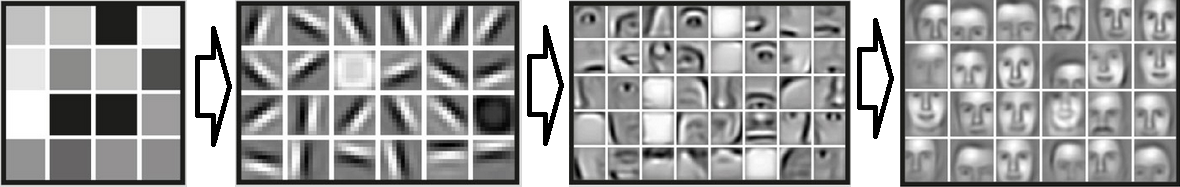
\includegraphics[width=0.7\linewidth]{./images/1_Features}
\caption[]{Partitionierung des Eingaberaums in unterschiedlichen Abstraktionsebenen (\textit{Distributed Representation}) (Andrew Ng, Stanford Artificial Intelligence Lab)}
\label{fig:1_Features}
\end{figure}
\end{center}
\begin{myblock}{Relevante Anwendungsfelder}
\begin{itemize}
\item Bilderkennung
\item Natürliche Sprache (NLP)
\item Robotik
\end{itemize}
\end{myblock}
\end{frame}

\begin{frame}[t]
\frametitle{Renaissance im Deep Learning}
\begin{itemize}
\item Bis 2006 keine nennenswerte Erfolge beim Training tiefer Architekturen
\item Ausnahme: Convolutional Neural Networks \\\textit{LeNet 5 von \cite{LeCun1998}}
\end{itemize}
\begin{myblock}{Durchbruch durch schichtweises Vortraining}
\begin{itemize}
\item \bibentry{Hinton2006}
\end{itemize}
\end{myblock}
\begin{itemize}
\item Verallgemeinerung auf $\mathbb{R}$ (\cite{Bengio2007})
\item Verallgemeinerung auf Bildausschnitte (\cite{Ranzato2006})
\end{itemize}
\end{frame}

\begin{frame}
\frametitle{Forschungsfelder im Deep Learning}
\begin{itemize}
\item Recurrent Neural Networks (RNN) 		\\ (\cite{Hochreiter1997})
\item Convolutional Neural Networks (CNN) 	\\ (\cite{LeCun1998})
\item Deep Belief Networks (DBN)				\\ (\cite{Bengio2007})
\item Stacked Denoising Autoencoders (SDA)	\\ (\cite{Vincent2008})
\item Deep Reinforcement Learning (DRL)		\\ (\cite{Mnih2013})
\end{itemize}
\end{frame}


%
% % % % % % % % % % % % % % % % % % % NEURONALE NETZE % % % % % % % % % % % % % % %
%
\section{Convolutional Neural Networks}
\begin{frame}
\begin{center}
\Huge Convolutional Neural Networks
\end{center}
\end{frame}

\begin{frame}
\frametitle{Multilayer Perceptrons (MLP)}
\begin{multicols}{2}
\begin{figure}
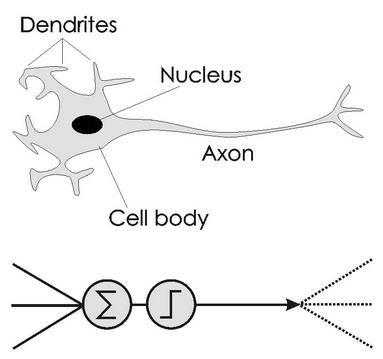
\includegraphics[width=0.3\textwidth]{images/2_neuron}
\caption{Schematischer Vergleich von biologischen und künstlichen Neuronen von \cite{McCulloch1943}}
\end{figure}
\begin{figure}
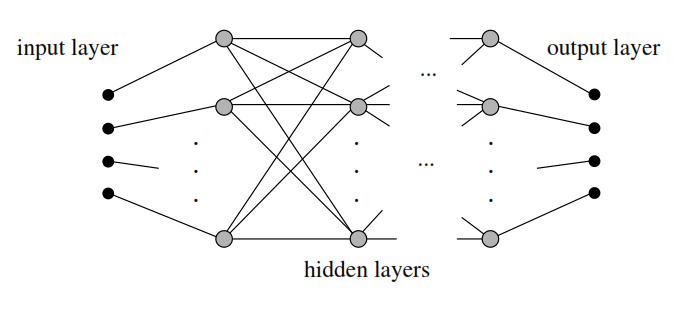
\includegraphics[width=0.5\textwidth]{images/2_mlp}
\caption{Generische mehrschichtige Architektur eines MLP (\cite{Rojas1996}) }
\end{figure}
\end{multicols}
\end{frame}

\begin{frame}
\frametitle{Multilayer Perceptrons (MLP)}
Einfachster Fall eines MLP:
\begin{itemize}
\item Ein Hidden-Layer $h$ mit einem Neuron
\item Ein Output-Layer $o$ mit einem Neuron
\end{itemize}
\begin{myblock}{Formale Beschreibung}
$f(x) = \phi(\langle w_o, \phi(\langle w_h, x \rangle + b_h) \rangle + b_o)$
\begin{itemize}
\item Eingabevektor $x$
\item Gewichtsvektor $w$
\item Schwellwert $b$
\item Aktivierungsfunktion $\phi(\cdot)$
\end{itemize}
\end{myblock}
\end{frame}

\begin{frame}
\frametitle{Logistische Sigmoid-Aktivierungsfunktion}
\begin{center}
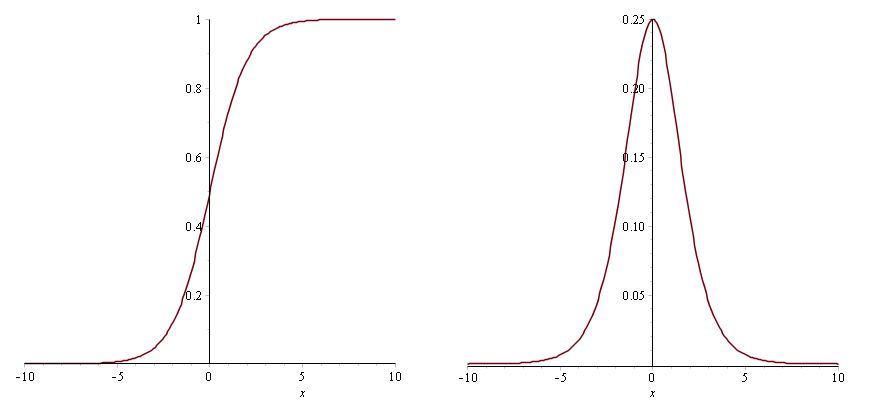
\includegraphics[width=0.6\textwidth]{images/2_sigmoid}
 \begin{itemize}
 \item Funktion: 
 $sig(x) = \frac{1}{1 + \exp^{-t}} $ 
 \item Ableitung: 
 $sig'(x) = sig(x)(1-sig(x))$
 \end{itemize}
\end{center}
\end{frame}


\begin{frame}
\frametitle{Backpropagation-Algorithmus}
\begin{itemize}
\item Verallgemeinerung der Delta-Regel im LMS-Algorithmus
\item Verfahren zur Berechnung partieller Ableitungen mittels Kettenregel (Fehlerrückführung) 
\end{itemize}
\begin{myblock}{Beispiel Output-Layer $L$}
Kostenfunktion: $J(W,b) = \frac{1}{2N} \sum_{i=1}^{N}(f(x_i) - y_i)^2$ \\
\vspace{0.2cm}
Delta-Regel: $\delta^{L} = (f(x_i) - y_i) \circ \phi'(z^{L})$ \\
\vspace{0.2cm}
Rückpropagierung: $\delta_{message}^{L} = (W^{L})^T \delta^{L}$
\end{myblock}
\begin{myblock}{Partielle Ableitungen Output-Layer $L$}
$\frac{\partial J(W,b)}{\partial W^L} = \frac{1}{N} \sum_{i=1}^{N} \delta^{L} (x_i^{L})^T$ \space \space\space\space
$\frac{\partial J(W,b)}{\partial b^L} = \frac{1}{N} \sum_{i=1}^{N} \delta^{L}$
\end{myblock}
\end{frame}

\begin{frame}
\frametitle{Beispiel Funktionsapproximation}
\begin{figure}
\centering
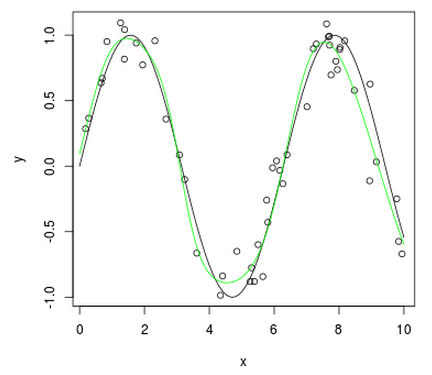
\includegraphics[width=0.5\textwidth]{images/2_sine_nn}
\caption{Approximierte Sinuskurve mit einem Hidden-Layer mit 6 Neuronen (grün)}
\end{figure}
\end{frame}


\begin{frame}
\frametitle{Beispiel Logistische Regression}
\begin{figure}
\centering
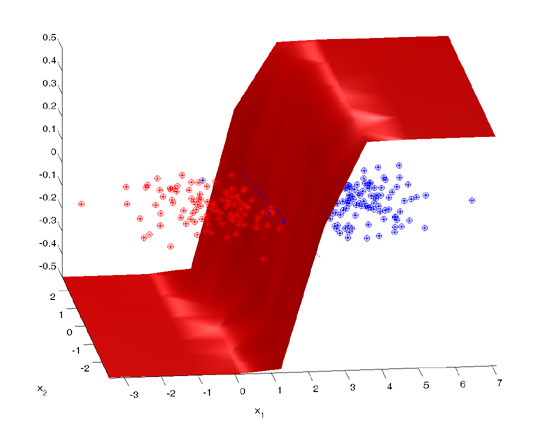
\includegraphics[width=0.6\textwidth]{images/2_logistic_regression}
\caption{Logistische Regression mit zwei Klassen (Vadim Strijov,
Computing Centre of the Russian Academy of Sciences)}
\end{figure}
\end{frame}

\begin{frame}
\frametitle{Output-Layer}
\begin{itemize}
\item Anzahl Neuronen im Output-Layer bestimmen Dimension der Ausgabe
\item Lineare Aktivierungsfunktion für Regression
\item Softmax-Regression für Klassifikation
\end{itemize}
\begin{myblock}{Kostenfunktion Logistische Regression}
$- ln(p(y|X,\hat{W})) = - \sum_{i=1}^N  y_i ln(f(x_i)) + (1-y_i) ln(1 - f(x_i))$ \\
\vspace{0.2cm}
mit $f(x_i) = \frac{1}{1 + \exp^{-\hat{W}x_i}} $
\end{myblock}
\begin{itemize}
\item Negative Log-Likelihood (Cross-Entropy-Fehlermaß)
\end{itemize}
\end{frame}




\begin{frame}
\frametitle{Convolutional Neural Networks (CNNs)}
\begin{itemize}
\item Spezielle Klasse von MLPs 
\item Zusätzliche Convolution-Layer mit \textit{Feature-Maps} als Ausgabe
\item Training mittels Backpropagation
\end{itemize}
\begin{myblock}{Berechnung einer \textit{Feature-Map} i im Convolution-Layer}
\begin{multicols}{2}
$z_i = \sum_{j=0}^{m}  x_{j} \ast W_{ij}$ \\
\vspace{0.3cm}
$a_{i} = \phi(z_{i} + b_i)$
$~$ \\ $~$ \\
\begin{itemize}
\item Eingabe $x$
\item Faltungsmaske $W_{ij}$
\item Schwellwert $b_i$
\item Aktivierungsfunktion $\phi(\cdot)$
\end{itemize}
\end{multicols}
\end{myblock}
\end{frame}

\begin{frame}
\frametitle{Lokales Rezeptives Feld}
\begin{figure}
\centering
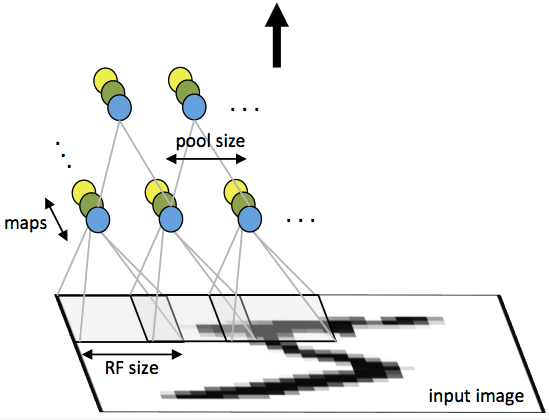
\includegraphics[width=0.6\textwidth]{images/3_Local_Receptive_Field}
\caption{Lokales Rezeptives Feld auf Basis der Entdeckungen von \cite{Wiesel1962} hinsichtlich des visuellen Cortex (\cite{Kaparthy2014})}
\end{figure}
\end{frame}


\begin{frame}
\frametitle{Convolution-Layer}
\begin{figure}
\centering
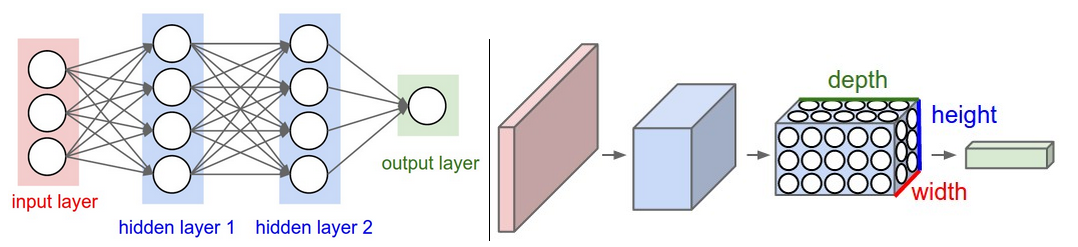
\includegraphics[width=0.9\textwidth]{images/3_cnn_kernel}
\caption{Beispiel Convolution-Layer (\cite{Kaparthy2014})}
\end{figure}
\end{frame}

\begin{frame}
\frametitle{Pooling-Layer}
\begin{figure}
\centering
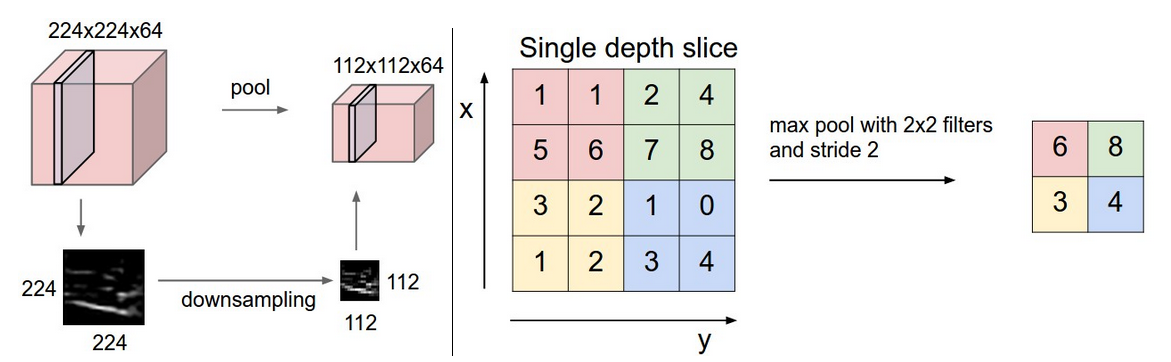
\includegraphics[width=0.9\textwidth]{images/3_cnn_subsampling}
\caption{Beispiel Max-Pooling-Layer (\cite{Kaparthy2014})}
\end{figure}
\end{frame}

\begin{frame}
\frametitle{Eigenschaften der CNN-Architektur}
\begin{itemize}
\item Lokale Extraktion von Merkmalen (\textit{Local Feature Extraction})
\item Translationsinvarianz hinsichtlich Eingabedaten (geringe Skalierungs- und Rotationsinvarianz)
\item Einfacheres Training durch weniger Parameter und Verbindungen als MLP mit gleich vielen Neuronen (\textit{Parameter Sharing})
\item Nicht-lokale Generalisierung durch Verschachtlung nichtlinearer Funktionen
\end{itemize}
(Vgl. \cite{LeCun1998}, \cite{Bengio2007b} und \cite{Zeiler2014}))
\end{frame}

\begin{frame}
\frametitle{Beispielarchitektur}
\begin{figure}
\centering
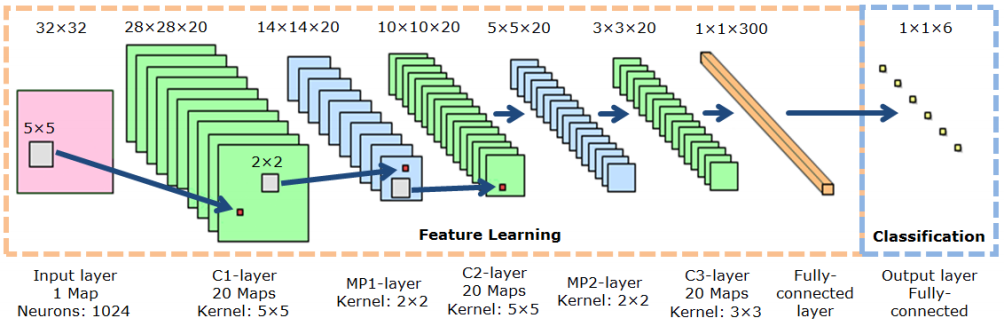
\includegraphics[width=0.9\textwidth]{images/3_CNN_Architecture}
\caption{Schematisches Convolutional Neural Network (\cite{Nagi2011})}
\end{figure}
\end{frame}


\begin{frame}
\frametitle{Beispielarchitektur: AlexNet}
\begin{figure}
\centering
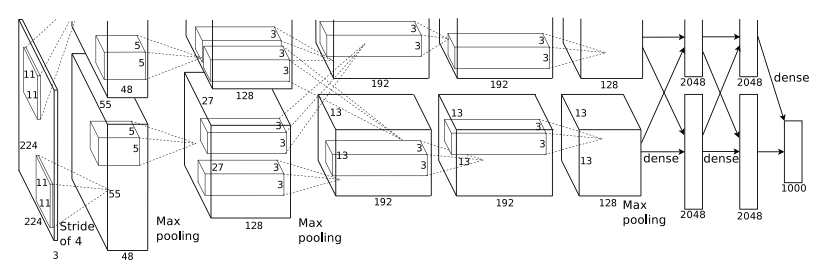
\includegraphics[width=1.0\textwidth]{images/4_Kriz}
\caption{Architektur von \cite{Krizhevsky2012} für ImageNet 2012 (Klassifikationsproblem mit 200 Klassen und 450.000 $482 \times 415$ Pixel großen Trainingsbeispielen)}
\end{figure}
\end{frame}



%
% % % % % % % % % % % % % % % % % % %  METHODEN % % % % % % % % % % % % % % % % % % 
%

\begin{frame}
\frametitle{Deep Learning und CNNs?}
\begin{figure}
\centering
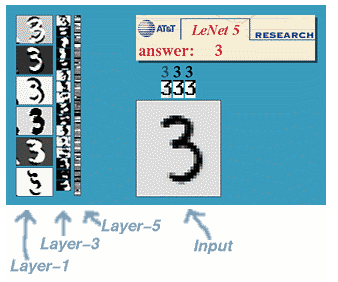
\includegraphics[width=0.3\textwidth]{images/3_lenet}
\caption{LeNet 5 von \cite{LeCun1998}}
\end{figure}
\begin{myblock}{Fehlerraten von LeNet 5 auf dem MNIST-Datensatz}
\begin{itemize}
\item 0.95 \% ohne erweiterten Trainingsdaten
\item 0.85 \% mit erweiterten Trainingsdaten
\item 20 Epochen Training (Iterationen über Trainingsset)
\end{itemize}
\end{myblock}
\end{frame}

\begin{frame}
\frametitle{Deep Learning und CNNs!}
Auch durch die Verwendung von CNNs bleiben dennoch zentrale Schwierigkeiten im Deep Learning bestehen:
\begin{itemize}
\item Verschwinden des Gradienten (\textit{Vanishing Gradient}) in tiefen Netzen (vgl. \cite{Hochreiter1991})
\item Gradientenabstieg bei nicht-konvexer Zielfunktion (vgl. \cite{Martens2010} und \cite{Dauphin14})
\item \textit{Overfitting} bei großen Netzen, insbesondere in nachgeschalteten MLPs (vgl. \cite{Hinton2012})
\end{itemize}
\end{frame}



\begin{frame}
\frametitle{Vanishing Gradient-Effekt}
\begin{figure}
\centering
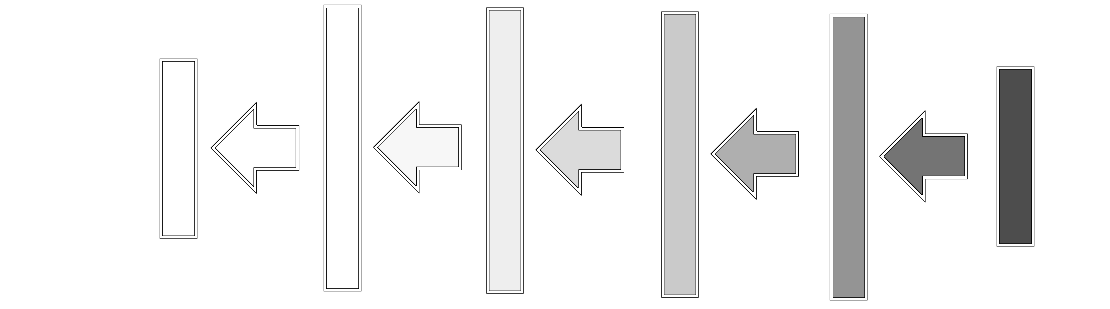
\includegraphics[width=0.5\textwidth]{images/4_vanishing_gradient}
\caption{Der Vanishing Gradient-Effekt beschreibt bei der
Rückpropagierung das abklingende Fehlersignal von Output- hin zu Input-Layer}
\end{figure}

\begin{myblock}{Backward-Pass im Backpropagation-Algorithmus}
$\delta_{message}^{l} = (W^{l})^T (\delta_{message}^{l+1} \circ \phi'(z^l)) $ 
\vspace{0.2cm} \\
mit $\phi'(z^l) <= 1 $
\end{myblock}

\end{frame}


\begin{frame}
\frametitle{Xavier-Initialisierung I}
\begin{itemize}
\item Normalisierte Signalpropagierung (Forward-Pass und Backward-Pass) von \cite{Glorot2010}
\item Zufällige Initialisierung mit unterschiedlicher Varianz pro Schicht
\item Wirkt dem Vanishing-Gradient-Effekt entgegen
\end{itemize}
\begin{myblock}{Formale Definition}
$W \sim \mathcal{U} [-\frac{\sqrt{6}}{\sqrt{fan_{in}  + fan_{out}}}, \frac{\sqrt{6}}{\sqrt{fan_{in}  + fan_{out}}}]$ \\
\vspace{0.2cm}
basierend auf $Var(W) = \frac{2}{fan_{in}  + fan_{out}}$
\end{myblock}
\end{frame}

\begin{frame}
\frametitle{Xavier-Initialisierung II}
\begin{figure}
\centering
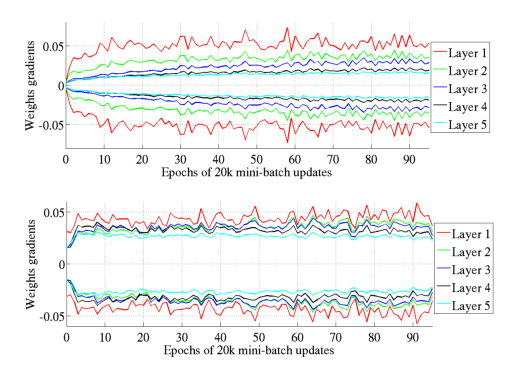
\includegraphics[width=0.6\textwidth]{images/4_xavier_init.PNG}
\caption{Vergleich der Varianz der Gradienten im Laufe des Trainings
(Standard-Initialisierung (oben) und Xavier-Initialisierung (unten)): Layer 1
entspricht dem Output-Layer mit der größten Varianz im Gradient (\cite{Glorot2010})}
\end{figure}
\end{frame}

\begin{frame}
\frametitle{ReLu-Aktivierungsfunktionen}
Rectified Linear Units (ReLus) können nicht sättigen und verhindern somit ein Verblassen des Fehlersignals (\cite{Glorot2011}). 
\begin{center}
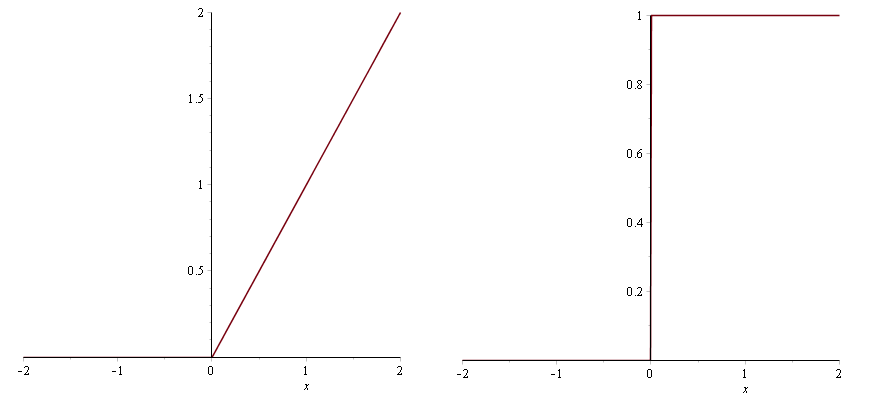
\includegraphics[width=0.6\textwidth]{images/2_relu}
   \begin{itemize}
   \item Funktion: 
   		$	f(x) =  max(0,x) $
   \item Ableitung: 
   		 $  f'(x) =
   		   \begin{cases}
   		     0 & \text{f"ur } 0 \ge x  \\
   		     1 & \text{f"ur } 0 < x
   		     \end{cases} $
   \end{itemize}
\end{center}
\end{frame}

\begin{frame}
\frametitle{Unüberwachtes Vortraining mittels Denoising Autoencoder}
\begin{figure}
\centering
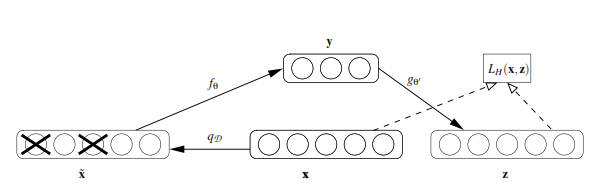
\includegraphics[width=0.7\textwidth]{images/4_vincent}
\caption{Schemadarstellung des Denoising Autoencoders (\cite{Vincent2010})}
\end{figure}
\begin{myblock}{Formale Definition}
$h = \phi(W\hat{x} + b)$ \\
\vspace{0.2cm}
$y = \phi(W'h + b')$
\vspace{0.2cm}
$ Loss = (x - y)^2 $
\end{myblock}
\end{frame}


\begin{frame}
\frametitle{Convolutional Autoencoder I}
\begin{myblock}{Verschiedene Herangehensweisen}
\begin{itemize}
\item Sequenzielle Verarbeitung von Bildausschnitten in Filtergröße und Training mittels Standard Autoencoder (vgl. \cite{Ranzato2006})
\item Berechnung aller Bildausschnitte gleichzeitig mittels Faltung und einem dem Backward-Pass ähnlichen Verfahren (vgl. \cite{Masci2011})
\end{itemize}
\end{myblock}
\begin{itemize}
\item Unüberwachtes Vortraining (schichtweise) führt zu einem besser konditionierten Lernproblem und kann so die Performanz verbessern
\item Bei CNNs, aufgrund von \textit{Parameter Sharing}, nicht so wirkungsvoll wie bei MLPs (\cite{Hamid2013})
\end{itemize}
\end{frame}


\begin{frame}
\frametitle{Convolutional Autoencoder II}
\begin{figure}
\centering
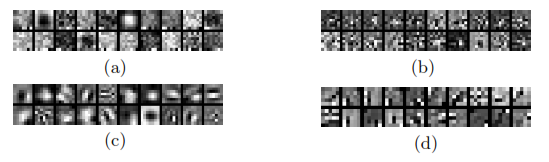
\includegraphics[width=0.7\textwidth]{images/4_mascii.PNG}
\caption{Filter der ersten Schicht eines Convolutional Autoencoders
(a) Kein Max-Pooling, 0 \% Rauschen, (b) Kein Max-Pooling, 50 \% Rauschen,
(c) Max-Pooling, (d) Max-Pooling , 30 \% Rauschen (\cite{Masci2011})}
\end{figure}
\end{frame}

\begin{frame}
\frametitle{Beispiel Fehlerlandschaft}
\begin{figure}
\centering
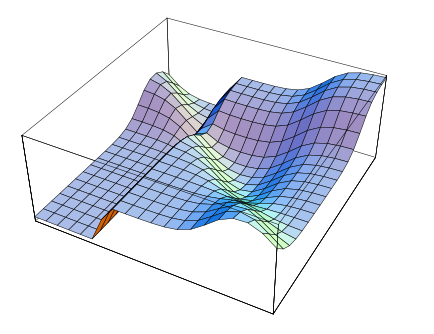
\includegraphics[width=0.6\textwidth]{images/4_Gradient2}
\caption{Fehlerfunktion beziehungsweise Zielfunktion im Gewichtsraum
mit lokalem Minimum (\cite{Rojas1996})}
\end{figure}
\end{frame}

\begin{frame}
\frametitle{Optimierung mittels Gradientenabstieg}
\begin{myblock}{Stochastischer Gradientenabstieg (SGD)}
$\nabla J(W,b) =  \mathbb{E}[\nabla (f(x_i) - y_i)^2] = \frac{1}{M}\sum_{i}^{M} \nabla (f(x_i) - y_i)^2$ \\
\vspace{0.2cm}
$W_{t+1} = W_t - \eta \frac{1}{M} \sum_{i=1}^{M} \nabla J(x_i)$ \\
\vspace{0.2cm}
mit Lernrate $\eta$ und M Trainingsbeispielen
\end{myblock}
\begin{itemize}
\item Online-Training: $M = 1$ 
\item Batch-Training: $M = N$ 
\item Averaged-SGD: $M \epsilon [1,N]$ (Mini-Batch)
\end{itemize}
\end{frame}

\begin{frame}
\frametitle{(Nesterov) Momentum-Methode}
\begin{figure}
\centering
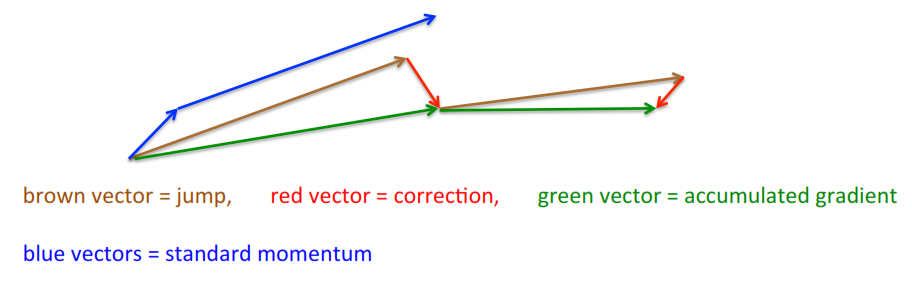
\includegraphics[width=0.6\textwidth]{images/4_nesterov}
\caption{Das Nesterov-Momentum korrigiert im Unterschied zur Momentum-Methode Fehler im
Nachhinein (\cite{Hinton2015})}
\end{figure}
\begin{myblock}{Formale Definition der Momentum-Methode}
$\Delta W_t = \mu \Delta W_{t-1} - \eta \nabla J(W_t,b_t)$ \\
\vspace{0.2cm}
$W_{t+1} = W_t + \Delta W_t$ \\
\vspace{0.2cm}
mit Momentum-Parameter $\mu$
\end{myblock}
\end{frame}

\begin{frame}
\frametitle{Adaptive Lernrate I}
\begin{myblock}{Newton-Schritt}
$W_{t+1} = W_t - H_t^{-1} \nabla J(W_t,b_t)$
\end{myblock}
\begin{itemize}
\item Quasi-Newton-Verfahren führt bei konvexen Zielfunktionen in zum globalen Minimum
\item Hesse-Matrix sehr teuer zu berechnen
\item \textbf{$\rightarrow$ Approximation der diagonalen Hesse-Matrix}
\end{itemize}
\end{frame}

\begin{frame}
\frametitle{Adaptiver Lernrate II}
Genannte Verfahren schätzen unterschiedliche Formen der diagonalen Hesse-Matrix: $|diag(H)|$, $\sqrt{diag(H)^2}$ oder $\sqrt{diag(H^2)}$ 
\begin{myblock}{Beispiele}
\begin{itemize}
\item Stochastischer LMA (\cite{LeCun1998b})
\item Rprop / RMSprop (\cite{Riedmiller1992} und \cite{Hinton2015})
\item AdaDelta (\cite{Zeiler2012})
\item Equilibrium SGD (\cite{Dauphin2015})
\end{itemize}
\end{myblock}
\end{frame}

\begin{frame}
\frametitle{RMSprop}
RMSprop approximiert $\sqrt{diag(H^2)}$  und stellt eine stochastische Variante von Rprop dar.
\begin{myblock}{Formale Definition}
$\hat{H}_{t+1} = \rho \hat{H}_{t} + (1 - \rho) \nabla J(W_t,b_t)^2$ \\
\vspace{0.2cm}
$\eta_{i} = \frac{\eta}{\mu + \sqrt{\hat{H}_{ii}}}$ \\
\vspace{0.2cm}
mit Faktor $\rho$ für exponentielle Glättung und Dämpfungsfaktor $\mu$
\end{myblock}
RMSprop bietet Vorteile bei einer Hesse-Matrix mit negativen Eigenwerten (Sattelpunkte) (\cite{Dauphin2015}).
\end{frame}


\begin{frame}
\frametitle{Overfitting}
\begin{figure}
\centering
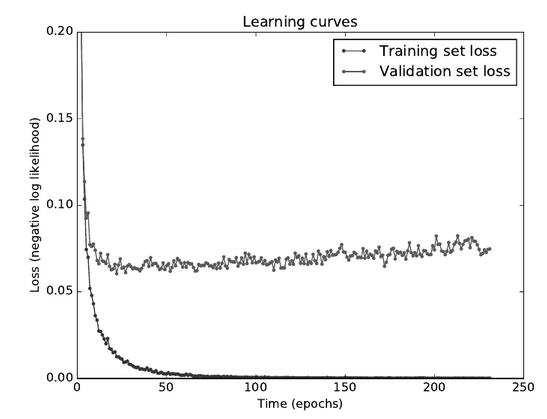
\includegraphics[width=0.6\textwidth]{images/4_overfitting.PNG}
\caption{Overfitting am Beispiel des MNIST-Datensatz (\cite{Bengio2015})}
\end{figure}
\end{frame}

\begin{frame}
\frametitle{Regularisierung}
Neben den bekannten Verfahren wie L1-/L2-Regularisierung (\textit{Weight Penalty}) oder Max-Norm-Regularisierung existieren im Bereich Deep Learning spezialisierte Verfahren:
\begin{myblock}{Spezielle Verfahren}
\begin{itemize}
\item Modellkapazität durch \textit{Parameter-Sharing} limitieren (CNNs).
\item Early-Stopping bricht Training bei Verschlechterung des Validierungsfehlers vorzeitig ab.
\item Erweiterung der Trainingsdaten durch additives Rauschen oder affinen oder elastischen Transformationen (\textit{Data Augementation})
\end{itemize}
\end{myblock}
\end{frame}

\begin{frame}
\frametitle{Dropout-Regularisierung}
\begin{figure}
\centering
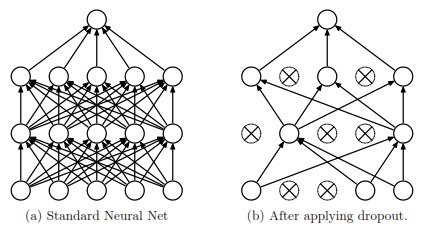
\includegraphics[width=0.8\textwidth]{images/4_dropout}
\caption{Schematische Darstellung eines gewöhnlichen MLP (links)
und eines Dropout-MLP (rechts) (\cite{Srivastava2014})}
\end{figure}
\end{frame}


%
% % % % % % % % % % % % % % % % % % %  IMPLEMENTIERUNG % % % % % % % % % % % % % % 
%


%\begin{frame}
%\frametitle{Vorverarbeitung}
%\centering
%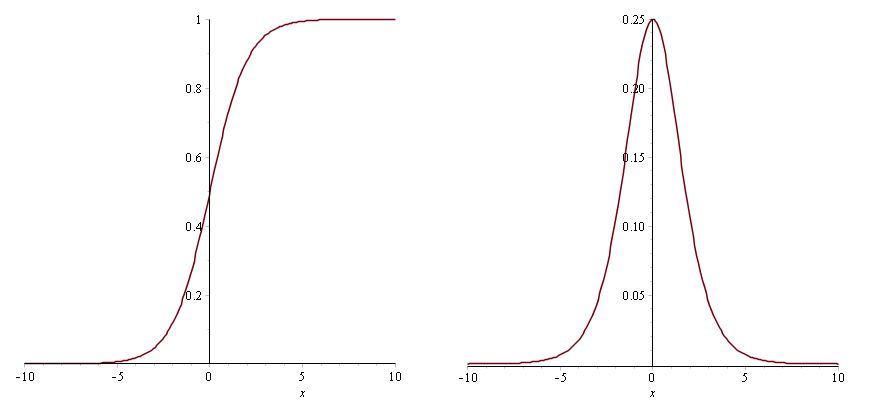
\includegraphics[width=0.6\textwidth]{images/2_sigmoid}
%\begin{itemize}
%\item Mittelwertfreie Trainingsdaten verhindern eine steile Fehlerlandschaft %(\cite{LeCun1998b}).
%\item Mittelwertfreie Trainingsdaten schließen Übersättigung der Aktivierungsfunktion %aus.
%\item Weitere Techniken sind Kontrastnormalisierung, Dekorrelation und (ZCA)-Whitening. 
%\end{itemize}
%\end{frame}


%
% % % % % % % % % % % % % % % % % % % EXPERIMENTE % % % % % % % % % % % % % % % % % %
%
\section{Experimente}
\begin{frame}
\begin{center}
\Huge Experimente
\end{center}
\end{frame}

%\begin{frame}
%\frametitle{Klassen-Abhängigkeitsgraph}
%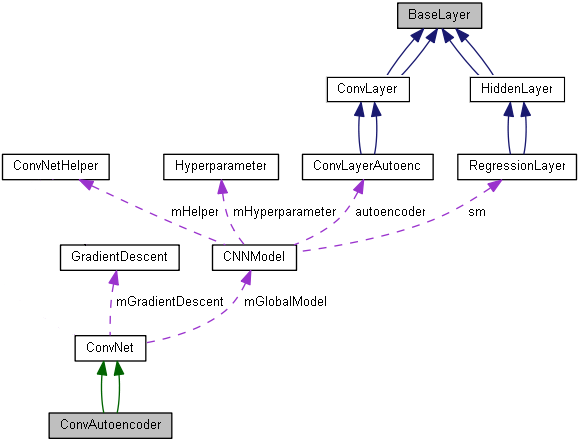
\includegraphics[width=0.8\textwidth]{images/5_class_hierarchie_autoencoder}
%\end{frame}



\begin{frame}
\frametitle{Betrachtete Datensätze I}
\begin{figure}
\centering
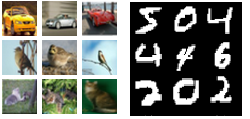
\includegraphics[width=0.5\textwidth]{images/experiments/6_samples}
\caption{Beispiele aus CIFAR-10 (links) und MNIST (rechts)}
\end{figure}
\end{frame}

\begin{frame}
\frametitle{Betrachtete Datensätze II}
\begin{myblock}{MNIST (Binarisierte handgeschriebene Ziffern)}
\begin{itemize}
\item 60000 $28 \times 28$ Pixel große Trainingsbeispiele sowie 10000 Testbeispiele. 
\item Richtwert für Fehlerrate ohne Vorverarbeitung liegt bei 0.7 \% (\cite{Ranzato2006}). 
\item Beste Ergebnis erreicht das \textit{DropConnect Network} von \cite{Zeiler2013} mit 0.21 \% Fehler.
\item Angewandte Vorverarbeitung: Zentrierung
\end{itemize}
\end{myblock}
\end{frame}

\begin{frame}
\frametitle{Betrachtete Datensätze III}
\begin{myblock}{CIFAR-10-Datensatz (Farbbilder)}
\begin{itemize}
\item 50000 $32 \times 32 $ Pixel große Trainingsbeispiele und 10000 Testbeispiele.
\item Die Bilder sind aufgeteilt in 10 Klassen.
\item Richtwert für Fehlerrate liegt bei 21.8 \% Fehler (\cite{Masci2011}). 
\item Bestes Ergebnis mit 8.2 \% Fehler erzielt das \textit{Deeply-Supervised Net} von \cite{Lee2014}.
\item Angewandte Vorverarbeitung: Zentrierung (CIFAR-10A (RGB) / CIFAR-10B (HSV))
\end{itemize}
\end{myblock}
\end{frame}

\begin{frame}
\frametitle{Architektur LeNet 5+ (MNIST)}
Die Netz ist ein erweitertes \textit{LeNet 5} und orientiert sich an dem von \cite{Ranzato2006} vorgestellten Modell.
\begin{myblock}{Layer-Definition}
\begin{enumerate}
\setlength{\itemsep}{0pt}
\item Convolution-Layer: 50 \textit{Feature-Maps} mit $5 \times 5$ Filtermasken
\item Pooling-Layer:	$2 \times 2$ Filtermasken
\item Convolution-Layer: 50 \textit{Feature-Maps} mit $5 \times 5$ Filtermasken
\item Pooling-Layer:	$2 \times 2$ Filtermasken
\item Hidden-Layer: 200 Neuronen
\item Output-Layer: 10 Neuronen mit Cross-Entropy Fehlermaß
\end{enumerate}
\end{myblock}
Dieses Netz umfasst 63.750 Gewichte in den Convolution-Layern und 162.000 Gewichte im MLP. 
\end{frame}

\begin{frame}
\frametitle{Architektur Net-7 (CIFAR-10)}
Dieses Netz orientiert sich an den Modellen von \cite{Hinton2012} und \cite{Zeiler2013b}.
\begin{myblock}{Layer-Definition}
\begin{enumerate}
\setlength{\itemsep}{0pt}
\item Convolution-Layer: 64 \textit{Feature-Maps} mit $5 \times 5$ Filtermasken
\item Pooling-Layer:	$2 \times 2$ Filtermasken
\item Convolution-Layer: 64 \textit{Feature-Maps} mit $5 \times 5$ Filtermasken
\item Pooling-Layer:	$2 \times 2$ Filtermasken
\item Convolution-Layer: 64 \textit{Feature-Maps} mit $5 \times 5$ Filtermasken
\item Hidden-Layer: 64 Neuronen
\item Output-Layer: 10 Neuronen mit Cross-Entropy Fehlermaß
\end{enumerate}
\end{myblock}
Dieses Netz umfasst 209.600 Gewichte in den Convolution-Layern und 10.496 Gewichte im MLP. 
\end{frame}

\begin{frame}
\frametitle{Trainingsmethode}
\begin{figure}
\centering

\includegraphics[width=0.5\textwidth]{images/experiments/6_validationset}
\end{figure}
\begin{itemize}
\item Early-Stopping mit 5 Epochen Wartezeit
\item 90\% Trainingsdaten und 10 \% Validierungsset
\item 40 Trainingsbeispiele pro Mini-Batch
\item Lernrate $\eta = 0.01$
\item Keine \textit{Data-Augmentation}
\end{itemize}
\end{frame}


\begin{frame}
\frametitle{Unüberwachtes Vortraining}
\begin{figure}
\centering
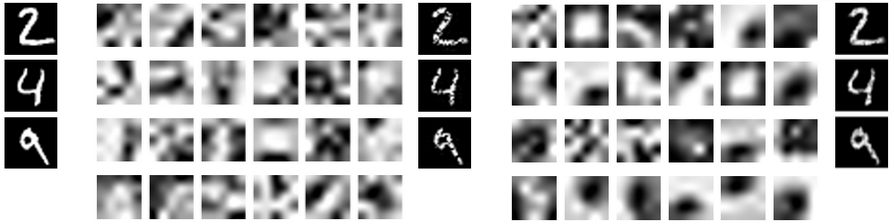
\includegraphics[width=0.8\textwidth]{images/experiments/6_mnist_autoencoder_combined}
\caption{Mittels Convolutional Autoencoder trainierte Filtermasken der ersten Schicht und erzeugte Rekonstruktionen: Ohne Maskierung (links) und mit 30 \% Maskierung (rechts).}
\end{figure}
\end{frame}


\begin{frame}
\frametitle{Klassifikation I}
\begin{table}
\centering
\begin{tabular}{c|c|c}
 	 			&   MNIST							& CIFAR-10B						 		\\ 
\hline SGD		&  0.40/0.82/0.93 \% (21)	&	\textcolor{green}{18.87/30.29/33.31 \% (27)}		\\
\hline Nesterov &  0.06/0.12/0.69 \% (11)	&	17.77/28.94/34.01 \% (34)				\\
\hline RMSprop  &  0.22/0.48/0.89 \% (10)	&	29.03/37.74/41.92 \% (29)				\\
\hline AdaDelta &  \textcolor{green}{0.02/0.18/0.61 \% (12)}	&	20.86/21.99/36.65 \% (12)				\\

%AdaDelta CIFAR 36.65
\end{tabular} 
\caption{Fehler auf den Trainings-/Validierungs-/Testdaten (Epochen) nach dem gesamten Training mit verschiedenen Methoden zum Gradientenabstieg}
\label{tab:6_gradientdescent}
\end{table}
\end{frame}


\begin{frame}
\frametitle{Klassifikation II (CIFAR-10B)}
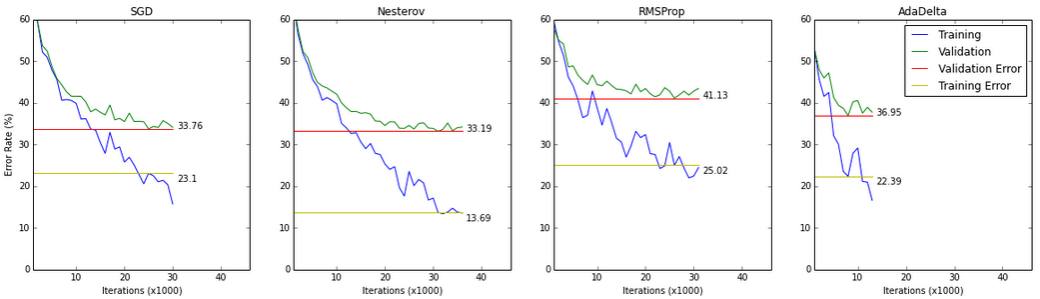
\includegraphics[width=1.0\textwidth]{images/experiments/6_training_cifar_2}
\end{frame}

\begin{frame}
\frametitle{Klassifikation mit Dropout (CIFAR-10B)}
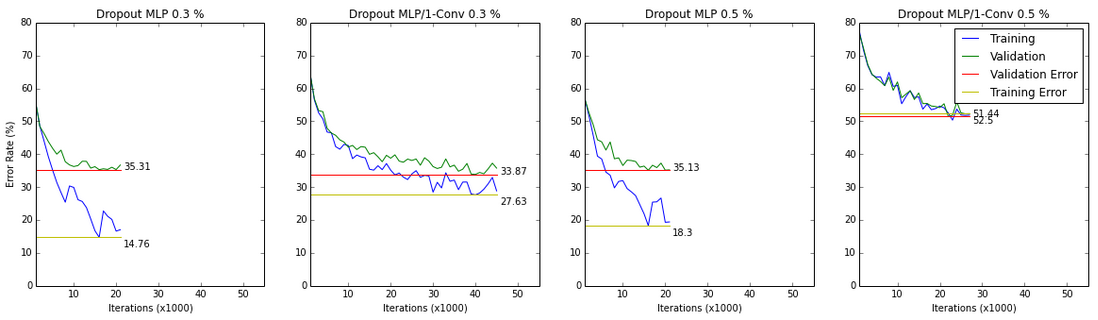
\includegraphics[width=1.0\textwidth]{images/experiments/6_overfit_dropout_2}
\end{frame}


\begin{frame}
\frametitle{Architektur Net-7-Small (CIFAR-10B)}
Entfernung von Hidden-Layer und Reduktion der Anzahl der \textit{Feature-Maps} auf 20 reduziert:
\begin{myblock}{Layer-Definition}
\begin{enumerate}
\setlength{\itemsep}{0pt}
\item Convolution-Layer: 20 \textit{Feature-Maps} mit $5 \times 5$ Filtermasken
\item Pooling-Layer:	$2 \times 2$ Filtermasken
\item Convolution-Layer: 20 \textit{Feature-Maps} mit $5 \times 5$ Filtermasken
\item Pooling-Layer:	$2 \times 2$ Filtermasken
\item Convolution-Layer: 20 \textit{Feature-Maps} mit $5 \times 5$ Filtermasken
\item Pooling-Layer:	$2 \times 2$ Filtermasken
\item Output-Layer: 10 Neuronen mit Cross-Entropy Fehlermaß
\end{enumerate}
\end{myblock}
 Insgesamt besitzt dieses Netz lediglich 24.700 Gewichte 
\end{frame}


\begin{frame}
\frametitle{Klassifikation Net-7-Small (CIFAR-10)}
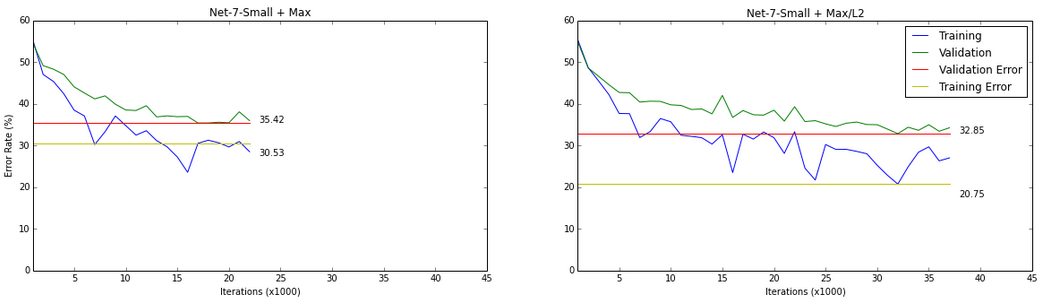
\includegraphics[width=0.9\textwidth]{images/experiments/6_overfit_small_2}
\end{frame}

 
\begin{frame}
\frametitle{Visualisierung der Filtermasken}
\begin{figure}
\centering
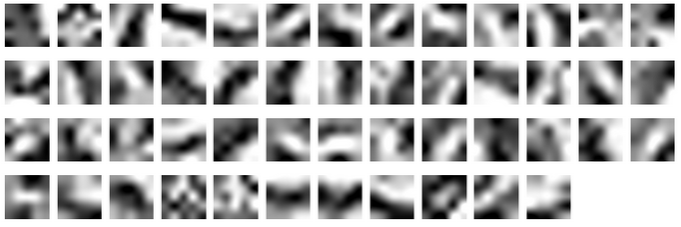
\includegraphics[width=0.8\textwidth]{images/experiments/6_mnist_trained_filters.png}
\caption{Filtermasken der ersten Schicht eines trainierten LeNet 5+}
\end{figure}
\end{frame}

\begin{frame}
\frametitle{Neuronen-Visualisierung}
\begin{figure}
\centering
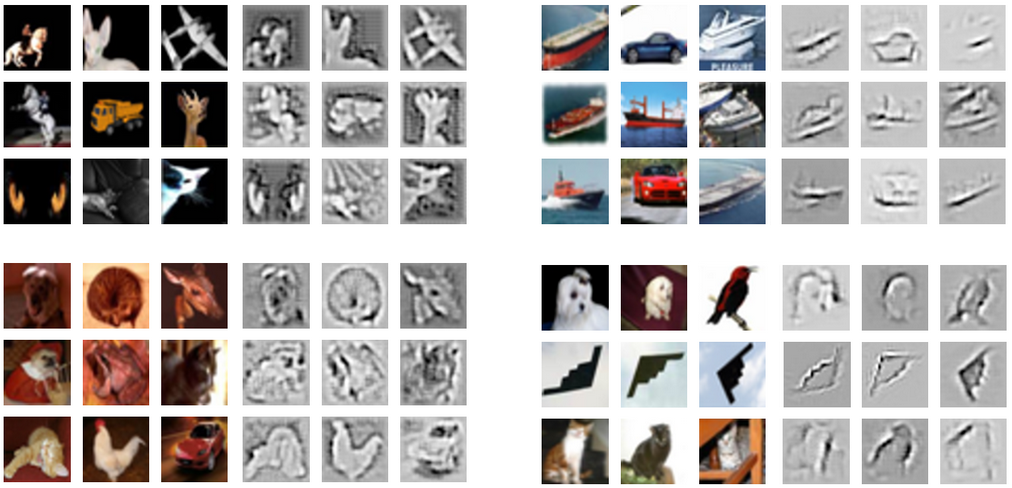
\includegraphics[width=0.8\textwidth]{images/experiments/6_visualize_cifar.png}
\caption{Visualisierung verschiedener Neuronen in der ersten Schicht (links) und in der zweiten Schicht (rechts) mittels der Methode von \cite{Zeiler2014}}
\end{figure}
\end{frame}


\begin{frame}
\frametitle{Autoencoder-Visualisierung}
\begin{figure}
\centering
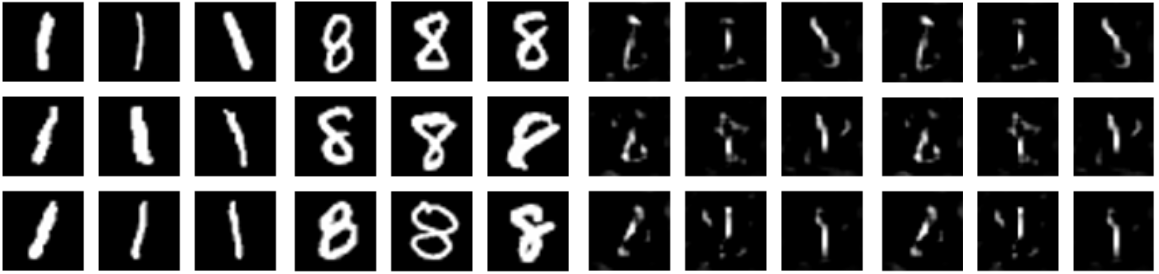
\includegraphics[width=0.8\textwidth]{images/experiments/6_visualize_mnist_autoenc_8_1}
\caption{Visualisierung kombinierter Merkmalsvektoren mittels Autoencoder}
\end{figure}
\end{frame}


\begin{frame}
\frametitle{t-SNE-Transformation MNIST}
\begin{figure}
\centering
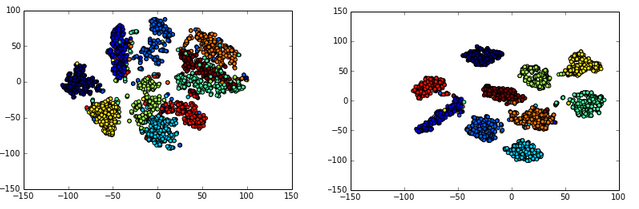
\includegraphics[width=0.8\textwidth]{images/experiments/6_tsne_mnist}
\caption{t-SNE-Encoding mit Originale (links) und mit CNN-Codes (rechts)}
\end{figure}
\end{frame}


%
% % % % % % % % % % % % % % % % % % % Ergebnisse % % % % % % % % % % % % % % % % % %
%

\section{Ergebnisse und Ausblick}
\begin{frame}
\begin{center}
\Huge Ergebnisse und Ausblick
\end{center}
\end{frame}


\begin{frame}[allowframebreaks]
\frametitle{Ergebnisse}
\begin{myblock}{Fehlerraten mit ConvNetCPP-Prototyp (AdaDelta-Methode)}
\begin{itemize}
\item 0.61 \% mit MNIST-Datensatz (12 Epochen)
\item 25.02 \% mit CIFAR-10-Datensatz (Padding) (72 Epochen)
\end{itemize}
\end{myblock}
\begin{itemize}
\item Padding erhöht die Kapazität und verbessert die Performanz ohne markant größeren Rechenaufwand.
\item Empfehlenswerte Optimierungsverfahren sind Nesterov-Momentum und AdaDelta-Methode.
\item Dropout und L2-Regularisierung sind gute Verfahren zur Verbesserung der Generalisierung.
\item Die Anwendung einer starken Regularisierung verlängert die Trainingszeit immens.
\item Ein kleiner dimensioniertes Netz kann gleichwertige Ergebnisse wie ein großes, nicht regularisiertes Netz erzielen.
\item Methoden zur Visualisierung sind gute Werkzeuge, um erlernte Merkmale sichtbar zu machen und die Funktionsweise von CNNs zu erklären.
\end{itemize}
\end{frame}


\begin{frame}[t]
\frametitle{Code Profiling}
Gemessene Laufzeiten des \textit{ConvNetCPP}-Prototyps:
\begin{itemize}
\item LeNet 5+ (MNIST)			$\approx 1 h$ CPU-Zeit pro Epoche \\
\item Net-7 (CIFAR-10)	\space	\space	$\approx 3 h$ CPU-Zeit pro Epoche	\\
\end{itemize}
\begin{myblock}{Laufzeitverhalten}
\begin{tabular}[t]{lrr@{.}l}
GEMM  							& 52 \%	\\
\texttt{img2col($\cdot$)} 		& 18 \% \\
\{=\}-Operator  				& 12 \%	\\
Speicherallokation 				& 8 \%	\\
\texttt{krnl2col($\cdot$)}		& 5 \%	\\
Sonstiges  						& 5 \%	\\
\end{tabular}
\end{myblock}
\end{frame}

\begin{frame}
\frametitle{General Matrix Multiply (GEMM)}
\begin{figure}
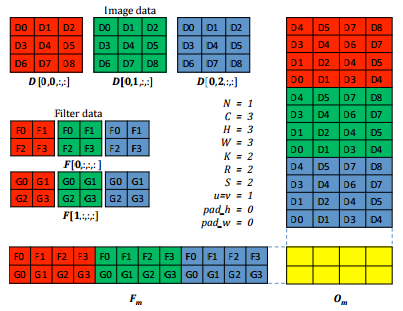
\includegraphics[width=0.6\textwidth]{images/5_convolution}
\caption{Reduktion der Faltung auf eine Matrix-Matrix-Multiplikation (GEMM) (\cite{Chetlur14}) }
\end{figure}
\end{frame}


\begin{frame}
\frametitle{Empfehlung für den Einsatz}
\begin{myblock}{Empfohlene Vorgehensweise}
\begin{enumerate}
\item Mit möglichst kleinem Netz starten
\item Sukzessive Erweiterung des Netzes bis der Validierungsfehler nicht weiter sinkt
\item Angleichung von Trainings- und Validierungsfehler mittels Techniken der Regularisierung für bestmögliche Generalisierung
\end{enumerate}
\end{myblock}
\end{frame}


\begin{frame}
\frametitle{Ausblick Prototyp}
\begin{multicols}{2}
\begin{itemize}
\item GPU-Implementierung
\item LC-Layer (Abb. rechts) \\ (\cite{LeRanzato2012})
\item Max-Out-Netze \\ (\cite{Goodfellow_maxout_2013})
\item Stacked Denoising Autoencoder \\ (\cite{Vincent2010})
\end{itemize}
\begin{figure}
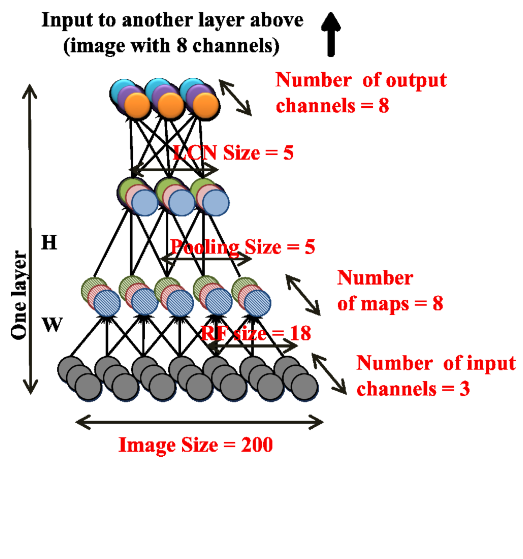
\includegraphics[width=0.5\textwidth]{images/4_ranzato}
%\caption{Google Autoencoder (\cite{LeRanzato2012})}
\end{figure}
\end{multicols}
\end{frame}

\begin{frame}
\frametitle{Ausblick Forschungsfeld}
\begin{myblock}{}
\begin{itemize}
\item Untersuchung von Transferlernen \\ (\textit{\cite{Bell2015} verwenden als Basis ein AlexNet})
\item Überwachung des Trainings \\ (\textit{\cite{Lee2014} verwenden SVMs pro Schicht})
\item Effizientere Verfahren zur Bestimmung von Hyperparametern
\item Entwicklung anderer Verfahren für das Lernen verteilter Repräsentationen
\end{itemize}
\end{myblock}

\end{frame}


%
% % % % % % % % % % % % % % % % %DISKUSSION % % % % % % % % % % % % % % % %
%


\section{Diskussion}
\begin{frame}
\frametitle{Diskussionsrunde}
\begin{center}
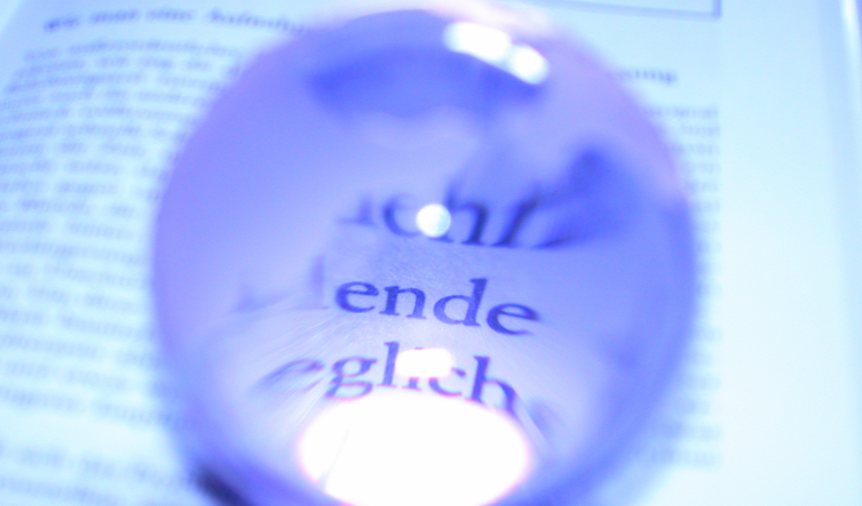
\includegraphics[width=0.9\textwidth]{images/Ende}
\end{center}
\end{frame}

\begin{frame}[allowframebreaks]
        \frametitle{Literatur}
        \bibliographystyle{bst_styles/apalike_german}
        %\bibliographystyle{plain}
        \bibliography{bibtex/literatur}
		%{\footnotesize\bibliography{bibtex/literatur}}
\end{frame}

\end{document}